\newpage
\section{Ergebnisse}
\label{sec:ergebnisse}
%5.) Inhalt des Kapitels: „Ergebnisse und Resultate
%- Darstellung der eigenen Versuchsergebnisse in Sätzen in Kombination mit
%entsprechenden Tabellen (u.a. aus Messprotokoll) und Abbildungen bzw. grafischer
%Darstellung der Ergebnisse.
%- Alle Abbildungen und Tabellen sind durchzunummerieren (Abb. 01, …, Tabelle 01: …)
%und mit einer Bild- bzw. Tabellenunterschrift zu versehen.
%- Der Inhalt von Abbildungen, z.B. der Verlauf eines Graphen, ist jeweils im Text zu
%erläutern und kurz zu beschreiben. Beschreibung der Verläufe von Funktionen bzw.
%der Graphen im Text unter Verweis auf die Abbildung bzw. Abbildungsnummer und
%Herausarbeitung ihrer „Kernaussage“ und Ursache bzw. Hintergründe besonderer
%„Verläufe“.
%- Rechenwege mit denen die experimentellen Daten für die Auswertung bearbeitet
%wurden bzw. der Gang der Auswertung muss vollständig beschrieben und für einen
%Leser nachvollziehbar sein.
\subsection*{Bestimmung der Stoffmengenanteile mittels Kalibrierung}
Zur Bestimmung der Ethanolanteile werden die gemessenen Brechungsindices, der flüssigen und gasförmigen Phase, mit Hilfe einer Kalibrierfunktion umgerechnet. Diese bestimmt sich durch die quadratische Regression der Daten, welche in der Versuchsanleitung gegeben sind. Gleichung \eqref{gl:reg} ist somit die Umrechnungsgleichung des Brechungsindexes in den jeweiligen Ethanol-Anteil.
\begin{flalign}
\label{gl:reg}
x_{\text{Ethanol}} (n)&= -97,53*n^2+256,05*n-166,86
\end{flalign}
Die sich daraus ergebenden Anteile sind in Tab. \ref{tab:zusammensetzung} aufgeführt. Es ist zuerkennen, dass die Werte für reines Ethanol und reines Cyclohexan nicht \SI{100}{\percent} entsprechen. Gründe hierfür könnten durch Messfehler verursacht werden und sollten in einer wiederholten Messung untersucht werden. Diese Abweichungen könnten die nachfolgenden Untersuchen und Schlussfolgerungen signifikant beeinflussen.
% Table generated by Excel2LaTeX from sheet 'Data'
\begin{table}[h!]
	\renewcommand*{\arraystretch}{1.2}
	\centering
	\caption{Brechungsindices und Zusammensetzungen der Flüssig- und Dampfphasen in Abhängigkeit von der Temperatur}
	\resizebox{15cm}{!}{
		\begin{tabular}{c|c|cc|cc|cc}
			\hline
			\textbf{Nr.} & $\boldmath T \left[\si{\celsius}\right]$ & $\boldmath n_{L} \left[-\right]$ &$\boldmath n_{V} \left[-\right]$ &$\boldmath x_{\text{\textbf{Ethanol}}}^L \left[-\right]$ &$\boldmath x_{\text{\textbf{Ethanol}}}^V \left[-\right]$ &$\boldmath x_{\text{\textbf{Cyclohexan}}}^L \left[-\right]$ &$\boldmath x_{\text{\textbf{Cyclohexan}}}^V \left[-\right]$ \\
			\hline
			1     & 78,709 & 1,359 & 1,358 & 0,996 & 1,005 & 0,004 & -0,005 \\
			2     & 74,350 & 1,360 & 1,375 & 0,987 & 0,826 & 0,013 & 0,174 \\
			3     & 71,380 & 1,365 & 1,383 & 0,938 & 0,723 & 0,062 & 0,277 \\
			4     & 69,444 & 1,368 & 1,387 & 0,907 & 0,667 & 0,093 & 0,333 \\
			5     & 68,168 & 1,371 & 1,391 & 0,873 & 0,607 & 0,127 & 0,393 \\
			6     & 67,277 & 1,374 & 1,393 & 0,838 & 0,576 & 0,162 & 0,424 \\
			7     & 66,160 & 1,381 & 1,395 & 0,750 & 0,545 & 0,250 & 0,455 \\
			8     & 77,996 & 1,423 & 1,42  & 0,019 & 0,082 & 0,981 & 0,918 \\
			9     & 73,657 & 1,422 & 1,413 & 0,040 & 0,224 & 0,960 & 0,776 \\
			10    & 70,381 & 1,422 & 1,408 & 0,040 & 0,319 & 0,960 & 0,681 \\
			11    & 68,180 & 1,420 & 1,406 & 0,082 & 0,356 & 0,918 & 0,644 \\
			12    & 65,943 & 1,414 & 1,402 & 0,204 & 0,427 & 0,796 & 0,573 \\
			13    & 65,374 & 1,407 & 1,401 & 0,338 & 0,445 & 0,662 & 0,555 \\
	\end{tabular}}
	\label{tab:zusammensetzung}%
\end{table}%
\FloatBarrier

\subsection*{Berechnung von Dampfdruck und Aktivitätskoeffizienten}
Die Berechnung der Dampfdrücke erfolgt nach der \textsc{Antoine}-Gleichung \eqref{gl:ant} und ist in umgestellter Form nach dem Dampfdruck in Gleichung \eqref{gl:ant_dampf} dargestellt. Die stoffspezifischen \textsc{Antoine}-Parameter sind der Versuchsanleitung zu entnehmen.
\begin{flalign}
\label{gl:ant_dampf}
p_i^0(T) \left[ \si{\kilo \pascal}\right]&= 10^{^{A-\frac{B}{C+T\, \left[\si{\celsius}\right]}}}
\end{flalign}
\newpage
Durch Umstellen der Gleichung \eqref{gl:rd} lässt sich nun mit Hilfe des Umgebungsdrucks und der ermittelten Stoffmengen Anteile, der jeweilige Aktivitätskoeffizient bestimmen. Dargestellt sind diese für Cyclohexan und Ethanol in Tab. \ref{tab:aktiv}. Die umgestellte Gleichung findet sich unter Gl. \eqref{gl:rd_um}. Der gemessene und korrigierte Umgebungsdruck belief sich im Versuch auf $p= \SI{100,841}{\kilo \pascal}$
\begin{flalign}
\label{gl:rd_um}
	\gamma_i &= \frac{p*x_i^V}{x_i^L*p_i^0(T)}
\end{flalign}

% Table generated by Excel2LaTeX from sheet 'Tabelle2'
\begin{table}[h!]
	\centering
	\renewcommand*{\arraystretch}{1.2}
	\caption{Dampfdrücke, Partialdrücke und Aktivitätskoeffizienten von Ethanol und Cyclohexan in Abhängigkeit von der Temperatur }
	\resizebox{15cm}{!}{
	\begin{tabular}{c|ccc|ccc}
		\hline
		$\boldmath T \left[\si{\celsius}\right]$ &$\boldmath p_{\text{\textbf{Ethanol}}}^0 \left[\si{\kilo \pascal}\right]$ & $\boldmath p_{\text{\textbf{Ethanol}}} \left[\si{\kilo \pascal}\right]$ & $\boldmath \gamma_{\text{\textbf{Ethanol}}} \left[-\right]$ &$\boldmath p_{\text{\textbf{Cyclohexan}}}^0 \left[\si{\kilo \pascal}\right]$ & $\boldmath p_{\text{\textbf{Cyclohexan}}} \left[\si{\kilo \pascal}\right]$ & $\boldmath \gamma_{\text{\textbf{Cyclohexan}}} \left[-\right]$ \\
		\hline
		78,709 & 102,361 & 101,345 & 0,994 & 95,315 & -0,504 & -1,322 \\
		74,350 & 85,610 & 83,295 & 0,986 & 83,300 & 17,546 & 16,203 \\
		71,380 & 75,586 & 72,908 & 1,028 & 75,819 & 27,933 & 5,942 \\
		69,444 & 69,605 & 67,261 & 1,065 & 71,235 & 33,580 & 5,069 \\
		68,168 & 65,889 & 61,210 & 1,064 & 68,336 & 39,631 & 4,566 \\
		67,277 & 63,395 & 58,084 & 1,093 & 66,367 & 42,757 & 3,977 \\
		66,160 & 60,383 & 54,958 & 1,214 & 63,962 & 45,883 & 2,869 \\
		77,996 & 99,444 & 8,269 & 4,376 & 93,262 & 92,572 & 1,012 \\
		73,657 & 83,175 & 22,588 & 6,789 & 81,505 & 78,253 & 1,000 \\
		70,381 & 72,447 & 32,168 & 11,101 & 73,426 & 68,673 & 0,974 \\
		68,180 & 65,923 & 35,899 & 6,641 & 68,362 & 64,942 & 1,035 \\
		65,943 & 59,813 & 43,059 & 3,529 & 63,503 & 57,782 & 1,143 \\
		65,374 & 58,338 & 44,874 & 2,276 & 62,312 & 55,967 & 1,357 \\
	\end{tabular}}
	\label{tab:aktiv}%
\end{table}%
\FloatBarrier	

\subsection*{Grafische Darstellung der Messergebnisse}
Für die grafische Auswertung der der experimentell ermittelten Daten wurde das Programm \textsc{VLE} verwendet. Die gemessenen Messpunkte werden in diesem Abschnitt mit den idealen Darstellungen des modifizierten \textsc{UNIFAC}-Modells verglichen.\\

In Abb. \ref{fig:siededia_unifac} ist die Temperatur des Systems in Abhängigkeit des Cyclohexan-Anteils dargestellt. Die blauen Linien beschreiben hierbei die Siedelinie und die grünen Linien stellen die Tauline dar. Die Farben der Messpunkte sind ebenfalls so zuzuordnen. Der Vergleich der Messpunkte mit den Kurvenverläufen zeigt geringfügige Abweichungen in Bezug auf das \textsc{UNIFAC}-Modell. Das spricht für die Plausibilität der Messwerte. Jedoch sollten für konkretere Aussagen wiederholte Messungen mit weiteren Zusammensetzungen geprüft werden. In dieser Darstellung ist zumindest der azeotrope Punkt des Gemisches deutlich zu erkennen und lässt sich in dieser Abbildung bei einer Temperatur von \SI{65}{\celsius} und einer Zusammensetzung von $x^L_\text{Cyclohexan}=0,55$ finden. 

\begin{figure}[h!]
	\centering
	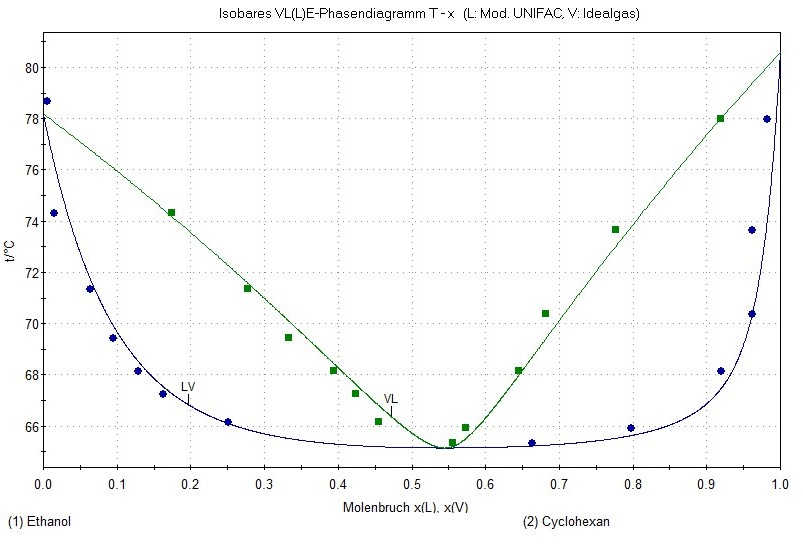
\includegraphics[width=0.75\textwidth]{img/Siededia_unifac}
	\caption{Messwerte und \textsc{UNIFAC}-Modell im Siedediagramm}
	\label{fig:siededia_unifac}
\end{figure}
\FloatBarrier
%Ende

In Abb. \ref{fig:ggw_unifac} sind die Dampfanteile von Cyclohexan in Abhängigkeit dessen Flüssiganteile in Form eines Gleichgewichtsdiagramms dargestellt. Die durchgezogene Linie entspricht dabei dem idealen Verlauf des Stoffgemisch nach \textsc{UNIFAC}-Modell und die Punkte den MEsswerten aus dem Praktikumsversuch. Auch an dieser Stelle sind geringe Abweichungen zu verzeichnen, welche jedoch im Sinne der idealen Gerade verlaufen. Auch zu erkennen ist der azeotrope Punkt, welcher als Schnittpunkt zwischen der Gleichgewichtsgeraden und der Diagrammdiagonalen zu verzeichnen ist. Die Plausibilität der Messwerte würde durch diese Darstellung ebenfalls gestützt werden.
\begin{figure}[h!]
	\centering
	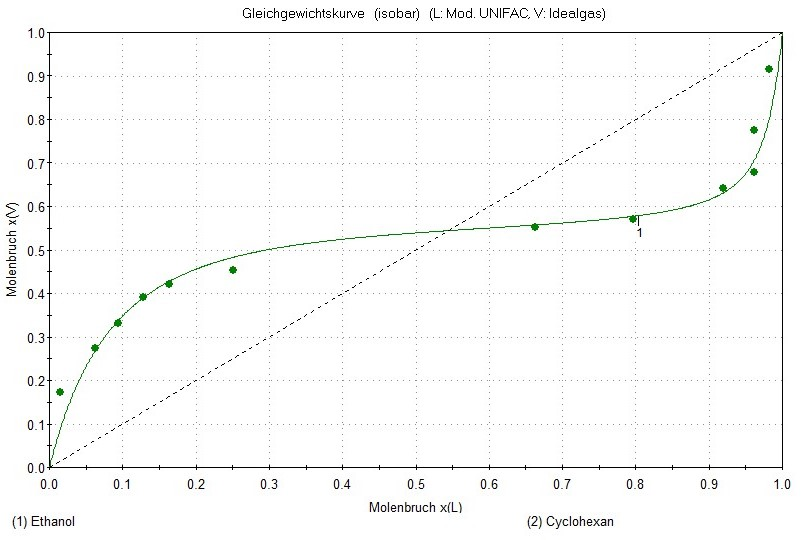
\includegraphics[width=0.75\textwidth]{img/GGW_unifac}
	\caption{Messwerte und \textsc{UNIFAC}-Modell im Gleichgewichtsdiagramm}
	\label{fig:ggw_unifac}
\end{figure}
\FloatBarrier
%Ende
In Abb. \ref{fig:gamma_unifac} sind die Aktivitätskoeffizienten des Ethanols und des Cyclohexans in Abhängigkeit des Molanteils an Cyclohexan in der Flüssigphase dargestellt. Die grüne Linie stellt dabei den Verlauf der Ethanol- und die blaue Linie den Verlauf der Cyclohexan-Aktivitätskoeffizienten dar. In dieser Abbildung fitten die Messwerte wieder größtenteils mit idealen Modell. Jedoch sind in dieser Darstellung deutliche Ausreißer zu verzeichnen, welche vor allem an den oberen und unteren Grenzwerten des Cyclohexan-Anteils zu finden sind. Diese sollten in erneuten Messungen überprüft werden. Sonst lässt sich feststellen, dass im Verlauf der Zunahme des Anteils an Cyclohexan in der Flüssigphase, der Aktivitätskoeffizientenverlauf von Ethanol steigt und der Verlauf von Cyclohexan gegenläufig sinkt.
\begin{figure}[h!]
	\centering
	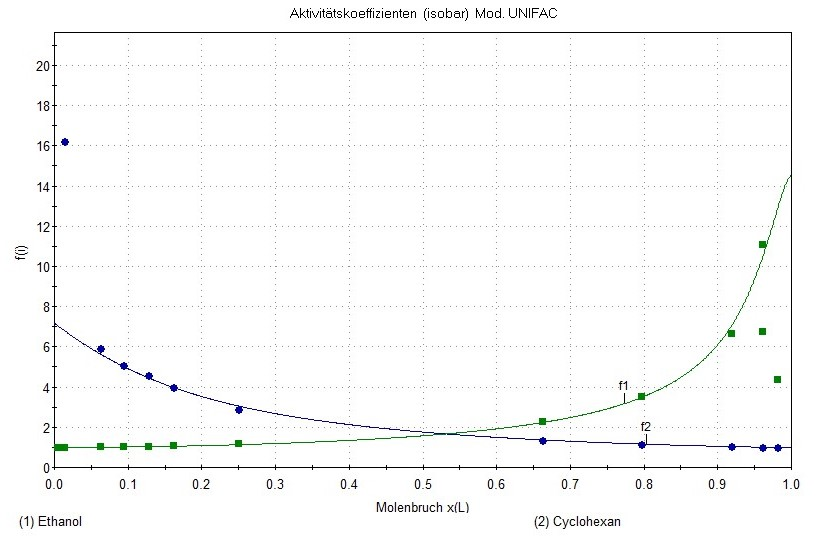
\includegraphics[width=0.75\textwidth]{img/gamma_unifac}
	\caption{Aktivitätskoeffizienten in Abhängigkeit Zusammensetzung der Flüssigphase der Messwerte und des \textsc{UNIFAC}-Modells}
	\label{fig:gamma_unifac}
\end{figure}
\FloatBarrier
%Ende

%\newpage

\subsection*{Berechnung der \textsc{Wilson}-Parameter}
Für die Berechnung der \textsc{Wilson}-Parameter und den sich daraus ergeben modellierten Daten in \textsc{VLE} ist zunächst die Bestimmung der Achsenabschnitte des folgenden Diagramms nötig:

\begin{figure}[h!]
		\begin{center}
			\resizebox{0.8\textwidth}{!}{
				\begin{tikzpicture}[trim axis left, trim axis right]
				\begin{axis}[
				%axis lines = left,
				width = 15cm,
				height = 11cm,
				xmin = 0,
				xmax = 1,
				ymin = -3,
				ymax = 3,
				%	ytick = {-4.5,-4,...,-1},
				%	xtick = {-10,-9,...,20},
				ylabel={$\ln \left(\frac{\gamma_{_\text{Cyclohexan}}}{\gamma_{_\text{Ethanol}}}\right)$},
				%y label style={at={(0,0.5)}},
				xlabel={$x^L_{\text{Cyclohexan}}$},
				legend style={at={(0.2,0.9)},anchor=west},
				%	y dir = reverse,
				]
				\addplot [color=black, mark=*, only marks] coordinates{(0.013,2.79953475724709) (6.20000000000001E-02,1.75414600797206) (0.093,1.55974753419804) (0.127,1.45656408409239) (0.162,1.29123260877454) (0.25,0.860542364306164) (0.96,-1.91526490817348) (0.96,-2.43310546327281) (0.918,-1.85903986852428) (0.796,-1.12724160875635) (0.662,-0.517226170435867)};
				
				\addplot +[mark=none, dashed, black, domain=0:5] {-4.420173865*x+2.18036538};
				
				\legend{berechnete Punkte, Regression mit $f(x) =\SI{ -4,42}{}*x+\SI{2,18 }{}\, | \, R^2= \SI{0,9725}{}$}
				\end{axis}
				\end{tikzpicture}}
			\caption{Logarithmisches Verhältnis der Aktivitätskoeffizienten in Abhängigkeit vom Stoffmengenanteil von Cyclohexan in der Flüssigphase}
			\label{dia:wilson_linear}
		\end{center}
	\end{figure}
	\FloatBarrier
	
	Das in Abb. \ref{dia:wilson_linear} dargestellte Diagramm zeigt die Messpunkte des logarithmierten Verhältnisses zwischen der Aktivität des Cyclohexans und der des Ethanols in Abhängigkeit von der Zusammensetzung des Anteils an Cyclohexan in der Flüssigphase. Zudem ist eine entsprechende Regressionsgerade mit einem Bestimmtheitsmaß on $R^2=0,9725$ eingezeichnet, welche für die Bestimmung der Achsenabschnitte benötigt wird. Mit dem ermittelten Bestimmtheitsmaß ist ein linearer Zusammenhang feststellbar, jedoch sollte eine erneute Messung in Erwägung gezogen werden um diesen Zusammenhang sachdienlich zu prüfen. Ebenso könnten für die Verbesserung des Bestimmtheitsmaßes statistische Ausreißer im größeren Maße aussortiert werden. \\
	Die ermittelten Achsenabschnitte sind in Tab. \ref{tab:abschnitt} dargestellt.
	\vspace*{-3mm}
	
% Table generated by Excel2LaTeX from sheet 'Daten'
\begin{table}[h!]
	\renewcommand*{\arraystretch}{1.2}
	\centering
	\caption{Achsenabschnitte $n_1$ und $n_2$}
	\label{tab:abschnitt}
		%\resizebox{10.5cm}{!}{
			\begin{tabulary}{1.0\textwidth}{C|C}
				\textbf{Achsenabschnitt} & \textbf{Wert}\\
				\hline
				\textbf{$n_{\text{Ethanol}} = \gamma^\infty_{\text{Ethanol}}$} &\SI{2,18}{}\\
				\textbf{$-n_{\text{Cyclohexan}} = \gamma^\infty_{\text{Cyclohexan}}$}&\SI{2,24}{}\\
				\hline		
	\end{tabulary}
%}
\end{table}%
\FloatBarrier

Die Berechnung der \textsc{Wilson}-Parameter $\Lambda_{12}$ und $\Lambda_{21}$ ist an dieser Stelle in den Gleichungen \eqref{gl:wilson_start} bis \eqref{gl:wilson_ende} aufgeführt.

\begin{flalign}
\label{gl:wilson_start}
	\ln (\Lambda_{12}) + \Lambda_{21} & = 1 - \gamma^\infty_{\text{Ethanol}}\\
																			&= 1- 2,18\\
																			&= \underline{-1,18}
\end{flalign}
\begin{flalign}
\ln (\Lambda_{21}) + \Lambda_{12} & = 1 - \gamma^\infty_{\text{Cyclohexan}}\\
&= 1- 2,24\\
&= \underline{-1,24}
\end{flalign}

\begin{flalign}
	\Lambda_{12} &= 1 - \gamma^\infty_{\text{Cyclohexan}}-\ln(\Lambda_{21})\\
	\ln(\Lambda_{21})&= \ln\left(1 - \gamma^\infty_{\text{Ethanol}}-\ln(\Lambda_{12})\right)\\
	\Lambda_{12} &= 1 - \gamma^\infty_{\text{Cyclohexan}}-\ln\left[1 - \gamma^\infty_{\text{Ethanol}}-\ln(\Lambda_{12})\right]\\
								&= 1-2,24-\ln(1-2,18-\ln(\Lambda_{12}))\\
								&= -1,24-\ln(-1,18-\ln(\Lambda_{12}))\\ \tag{iterativ gelöst}
								&= \underline{0,245}
\end{flalign}

\begin{flalign}
\label{gl:wilson_ende}
	\Lambda_{21} &= 1 - \gamma^\infty_{\text{Ethanol}}-\ln(\Lambda_{12})\\
								&= 1- 2,18-\ln(0,245)\\
								&=\underline{0,227}
\end{flalign}

Die berechneten \textsc{Wilson}-Parameter können nun im Programme \textsc{VLE} eingegeben werden. In den Abbildungen \ref{fig:siededia_wilson}, \ref{fig:ggw_wilson} und \ref{fig:gamma_wilson} sind die verschiedenen grafischen Darstellungen mit dem \textsc{Wilson}-Modell erfasst worden.\\

Im Siedediagramm nach \textsc{Wilson} ist zuerkennen, dass ein guter Fit der Messwerte erfolgt, jedoch subjektiv scheint es als wäre dieser Fit ungenauer als der des \textsc{UNIFAC}-Modells. Für genauere Bewertungen in dieser Richtung sollten die Abweichungen beider Modelle für die  Messwerte bestimmt und verglichen werden. 

\begin{figure}[h!]
	\centering
	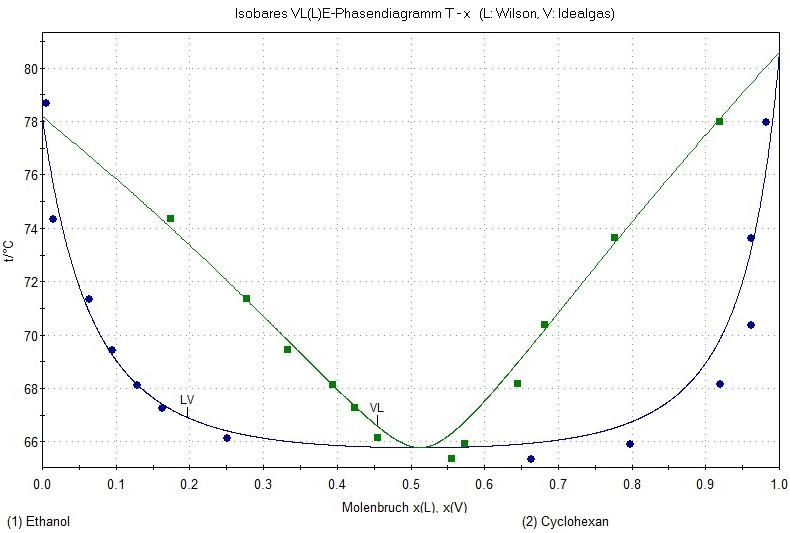
\includegraphics[width=0.75\textwidth]{img/siededia_wilson}
	\caption{Messwerte und \textsc{Wilson}-Modell im Siedediagramm}
	\label{fig:siededia_wilson}
\end{figure}
\FloatBarrier
%Ende

Im Gleichgewichtsdiagramm mit \textsc{Wilson}-Modell ist ebenfalls ein guter Fit des Graphen an die Messwerte zu erkennen, jedoch scheint auch hier rein optisch das \textsc{UNIFAC}-Modell geringfügig besser an den Messpunkten anzuliegen.

\begin{figure}[h!]
	\centering
	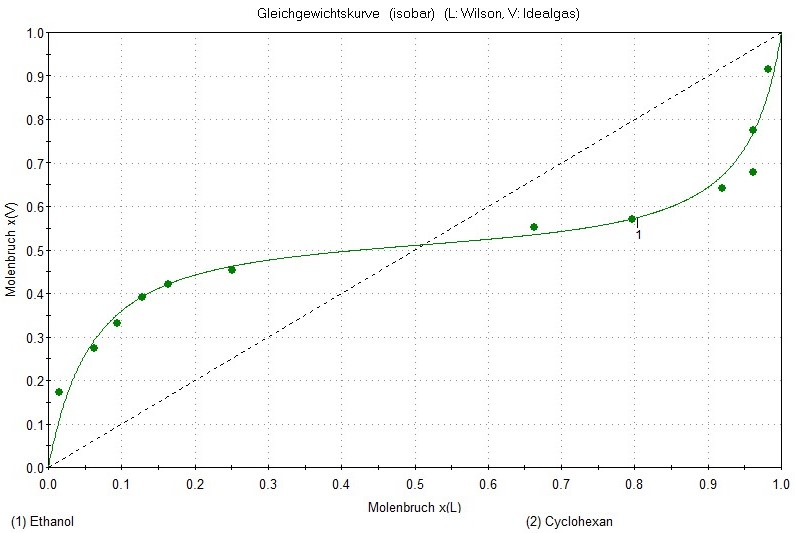
\includegraphics[width=0.75\textwidth]{img/GGW_wilson}
	\caption{Messwerte und \textsc{Wilson}-Modell im Gleichgewichtsdiagramm}
	\label{fig:ggw_wilson}
\end{figure}
\FloatBarrier
%Ende

In Abb. \ref{fig:gamma_wilson} zeigt sich nun im Vergleich zum \textsc{UNIFAC}-Modell ein besserer Fit der Aktivitätskoeffizientenverläufe. Zwar werden dennoch nicht alle scheinbaren Ausreißer im Modell erfasst, jedoch erfolgt, im Bereich gegen \SI{100}{\percent} Cyclohexan in der Flüssigphase, ein besserer Fit für die Aktivitätskoeffizienten des Ethanols.

\begin{figure}[h!]
	\centering
	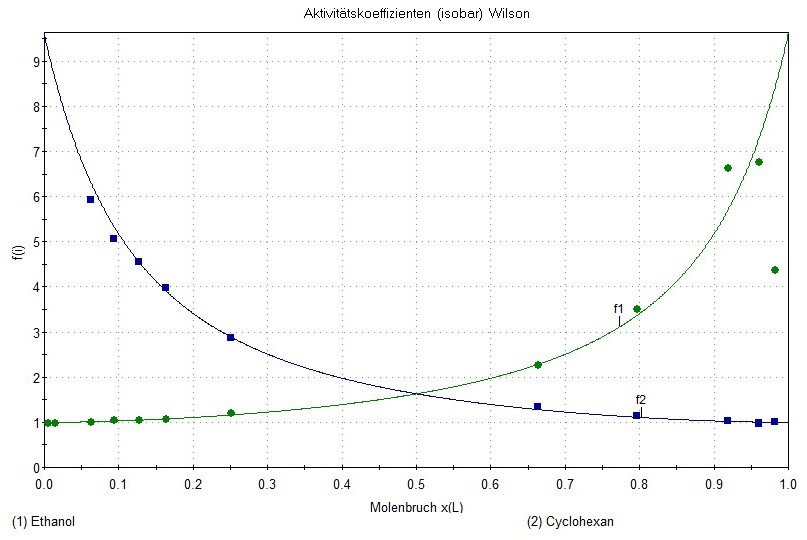
\includegraphics[width=0.75\textwidth]{img/gamma_wilson}
	\caption{Aktivitätskoeffizienten in Abhängigkeit Zusammensetzung der Flüssigphase der Messwerte und des \textsc{Wilson}-Modells}
	\label{fig:gamma_wilson}
\end{figure}
\FloatBarrier
%Ende

Aufgrund des Arbeitsaufwandes und der Genauigkeit des Fits in Bezug auf die gemessenen Daten im Praktikum würde man sich vermutlich tendenzielle eher für das \textsc{UNIFAC}-Modell als für das \textsc{Wilson}-Modell entscheiden. Diese Wertung ist jedoch nur für dieses Protokoll repräsentativ.